%***********************************************************************************************************************************************
\chapter[Gaussian Process Metamodeling]{Gaussian Process Metamodeling: Emulating Code Input/Output for Faster Evaluation}\label{ch:gp_metamodel}
%***********************************************************************************************************************************************

Under Bayesian calibration framework, tens, if not hundreds, of thousands code runs are to be expected to appropriately explore the posterior probability distribution using different values of parameters.
Such number of runs are only feasible for simulation with a negligible running time.
Therefore, to balance the need for vast number of code runs with the finite computing resources and time, 
an alternative approach is required to approximate the input/output relationships of the code for the selected relevant outputs within a selected input domain of interest. 

This chapter describes an approach to construct a fast surrogate model (metamodel) that approximates (or emulate) the input/output relationship of an expensive code for faster evaluation at any given input parameters values located in the specified domain.
As argued in Section~\ref{sub:intro_statistical_metamodeling} this thesis used the one based on Gaussian stochastic process, which results in a statistical metamodel. 

A statistical framework of metamodeling along with necessary notational conventions are first presented in Section~\ref{sec:gp_statistical_framework}.
The framework casts the problem of metamodeling as a problem of nonlinear regression where a set of limited actual code runs (with input parameters values judiciously selected) is used to predict code output at any other input values.

Afterward, a review on some fundamental concepts of multivariate Gaussian random variable and Gaussian stochastic process is presented in Section~\ref{sec:gp_fundamentals}.
The section also establishes an intuitive connection between multivariate Gaussian random variable and Gaussian stochastic process.
Section~\ref{sec:gp_metamodeling} then presents the formal Gaussian stochastic process formulation used for metamodeling followed by the important aspects of constructing it in Section~\ref{sec:gp_construction}.
Section~\ref{sec:gp_dimension_reduction} specifically deals with an approach to tackle the case of code with multiple outputs.

The application of the metamodeling approach to the \gls[hyper=false]{trace} model of the \gls[hyper=false]{feba} facility is given in Section~\ref{sec:gp_application_to_feba}.
The suitability of Gaussian process metamodel on the \gls[hyper=false]{trace} model is assessed using different choices made during the metamodel construction.
The results and important findings of this step are subsequently presented and briefly discussed.
Finally, Section~\ref{sec:gp_chapter_summary} summarizes the chapter.

%******************************************************************
\section{Statistical Framework}\label{sec:gp_statistical_framework}
%******************************************************************

Consider a general \emph{regression} problem:
\marginpar{regression problem}
Given a deterministic computer simulator (which, in essence, is a function) $f:\mathbf{x} \in \mathcal{X} \subseteq \mathbb{R}^D \mapsto \mathbb{R}$ 
evaluated at $\mathbf{DM}$, an experimental design matrix $\{\mathbf{x}_n\}_{n=1}^N$,
yielding $N$ outputs $\mathbf{y} = \{f(\mathbf{x}_n) = y_n\}_{n=1}^N$. 
the objective of regression is to compute (or \emph{predict}) the value of $f(\mathbf{x}_o)$ with $\mathbf{x}_o \notin \mathbf{DM}$.

The set $\mathcal{D} \equiv \{(\mathbf{DM}, \mathbf{y})\} = \{(\mathbf{x}_n, f(\mathbf{x}_n) = y_n)\}_{n=1}^N$ of $N$ observations is often referred to as the training data,
\marginpar{training data, training samples, and training outputs}
though the term is used interchangeably with the training outputs $\mathbf{y}$.
The experimental design matrix $\mathbf{DM}$ introduced in the previous chapter is interchangeably referred to as the training samples, inputs, or points in this chapter.
As before, the domain $\mathcal{X}$ is often rescaled such that $\mathbf{x} \in [0,1]^D$.

To evaluate $f$ at any given $\mathbf{x}_o \notin \mathbf{DM}$, the code of course can be simply run at that input.
\marginpar{emulator, surrogate model, and metamodel} 
Unfortunately, the true underlying function $f(\circ)$ that produces $y_i$ itself might be too complex and expensive to evaluate.
As such, the response surface of the function has to be reconstructed or estimated based only on small size of training data before the prediction is made.
The estimated function is chosen to be a simpler function that can be evaluated much faster (such as polynomials).
Although simpler, such an approximation should capture the most, if not all, important aspects of the inputs/outputs relationship of the true underlying function.
This simpler, approximating function is often referred to as an \emph{emulator}, \emph{surrogate model}, or \emph{metamodel}.

% Adopted framework
In this thesis, 
\marginpar{Gaussian process metamodel}
the metamodel is represented using \gls[hyper=false]{gp}, following the seminal works of Sacks et al. (\cite{Sacks1989, Sacks1989a}) and interpreted through a Bayesian perspective.
The advantages of using \gls[hyper=false]{gp} to represent an unknown function are its ability to model a complicated multi-dimensional function with limited number of parameters (\cite{Jones2009})
as well as the provision of prediction error estimate (\cite{Santner2003,Currin1991}).
Furthermore, being a statistical model based on a stochastic process, it fits the statistical calibration framework of computer model presented in the next chapter.

% Two Interpretations
The \gls[hyper=false]{gp} metamodel, like many statistical models, can be interpreted either in frequentistic sense or Bayesian sense.
\marginpar{Two interpretations}
In the frequentistic sense, the stochastic process $Y(\circ)$ is one particular realization of stochastic process (need not be Gaussian, but second-order stationary).
The prediction made at particular value of $\mathbf{x}_o$ is made based on the process as estimated according to the training data\footnote{The frequentistic case is the classical approach first developed as spatial interpolation tool in geostatistics by Krige dating back to the 1950s \cite{Krige1951} and formalized by Matheron in the 1960s \cite{Matheron1963}. In fact, Kriging model (due to Krige) is the more popular term for \gls[hyper=false]{gp} metamodel. These two terms, Kriging model and \gls[hyper=false]{gp} metamodel, will be used interchangeably in this thesis.}.
On the other hand, in the Bayesian sense, a Gaussian process is first set up as the prior for the stochastic process and the
prediction of the output at $\mathbf{x}_o$ is made based on the posterior (or conditional) process as updated by the training data.   

Both of these interpretations give an equivalent results.
The subtle difference lies in the interpretation of prediction error.
In the frequentistic case, the error is defined as the mean squared of error between the prediction made by the estimated process and (hypothetical) true process \cite{Isaaks1989};
\marginpar{prediction error}
while in the Bayesian case the error corresponds to the \emph{epistemic} uncertainty of the prediction conditional on the observed data.
That is, though the underlying computer simulation itself might be deterministic, 
the uncertainty of the prediction at $\mathbf{x}_o$ stems from the fact that the simulator was not actually run at that input and thus the output is not \emph{known}. 
The Bayesian perspective, as argued in \cite{Currin1991,Santner2003,OHagan2006}, gives more intuitive interpretation of the prediction error.
This perspective is illustrated in Fig.~\ref{fig:plot_bayesian_perspective}.
\bigtriplefigure[pos=tbhp,
								 mainlabel={fig:plot_bayesian_perspective},
			           maincaption={Gaussian process prior is equivalent to setting prior over functions. After observing data the process is updated to obtain the posterior process with a reduced uncertainties. Uncertainties are attached to each prediction made at arbitrary input outside the data (red points). Dashed lines and gray region signify the mean and $3\times \sigma$, respectively. The scales in the axes are arbitrary.},
			           mainshortcaption={Illustration of Bayesian perspective of regression and metamodeling.},%
			           leftopt={width=0.30\textwidth},
			           leftlabel={fig:plot_bayesian_perspective_1},
			           leftcaption={Prior of functions},
			           midopt={width=0.30\textwidth},
			           midlabel={fig:plot_bayesian_perspective_2},
			           midcaption={Observed data},
			           rightopt={width=0.30\textwidth},
			           rightlabel={fig:plot_bayesian_perspective_3},
			           rightcaption={Posterior function and predictions},
			           spacing={},
			           spacingtwo={}]
{../figures/chapter4/figures/plotBayesianPerspective_1}
{../figures/chapter4/figures/plotBayesianPerspective_2}
{../figures/chapter4/figures/plotBayesianPerspective_3}

\section{Gaussian Process Fundamentals}\label{sec:gp_fundamentals}

This section reviews the basics of \gls[hyper=false]{gp}.
The connection between the stochastic process and multivariate Gaussian random variable (Gaussian random vector) is first established.
Appendix~\ref{app:probability} gives some the basic concepts of multivariate random variable such as joint, marginal, and conditional probabilities.

\subsection[From Multivariate Gaussian to Gaussian Process]{From Multivariate Gaussian to Gaussian Process}\label{sub:gp_mvn}

% Illustration of Joint, Marginal, and Conditional
To illustrate the notions of joint, marginal, and conditional distributions, an example of a bivariate random variable, a random vector $Z = [Z_1, Z_2] \in \mathbb{R}^2$ is given.
\marginpar{random vector, an example}
It has the following mean vector and variance-covariance matrix, respectively,
\begin{equation}
	\begin{split}
		\begin{pmatrix}
			Z_1 \\
			Z_2
		\end{pmatrix} & \sim \mathcal{N}(\boldsymbol{\mu}, \boldsymbol{\Sigma}) \\
		 \boldsymbol{\mu} & = [0, 0]^T \\
		  \boldsymbol{\Sigma} = 
				\begin{pmatrix}
					\mathbf{V}[\mathbf{Z}_1]                & \text{Cov}[\mathbf{Z}_1, \mathbf{Z}_2]\\
					\text{Cov}[\mathbf{Z}_2, \mathbf{Z}_1]  & \mathbf{V}[\mathbf{Z}_2]\\
			\end{pmatrix} & =
			\begin{pmatrix}
					0.5       & -0.265165\\
					-0.265165 & 0.25\\
			\end{pmatrix}
	\end{split}
\label{eq:ex_bivariate}
\end{equation}
The joint, marginal, and conditional probability distributions of random vector $\mathbf{Z}$ are illustrated in Fig.~\ref{fig:plot_bivariate_normal}.
\begin{figure}[bth]
	\centering
	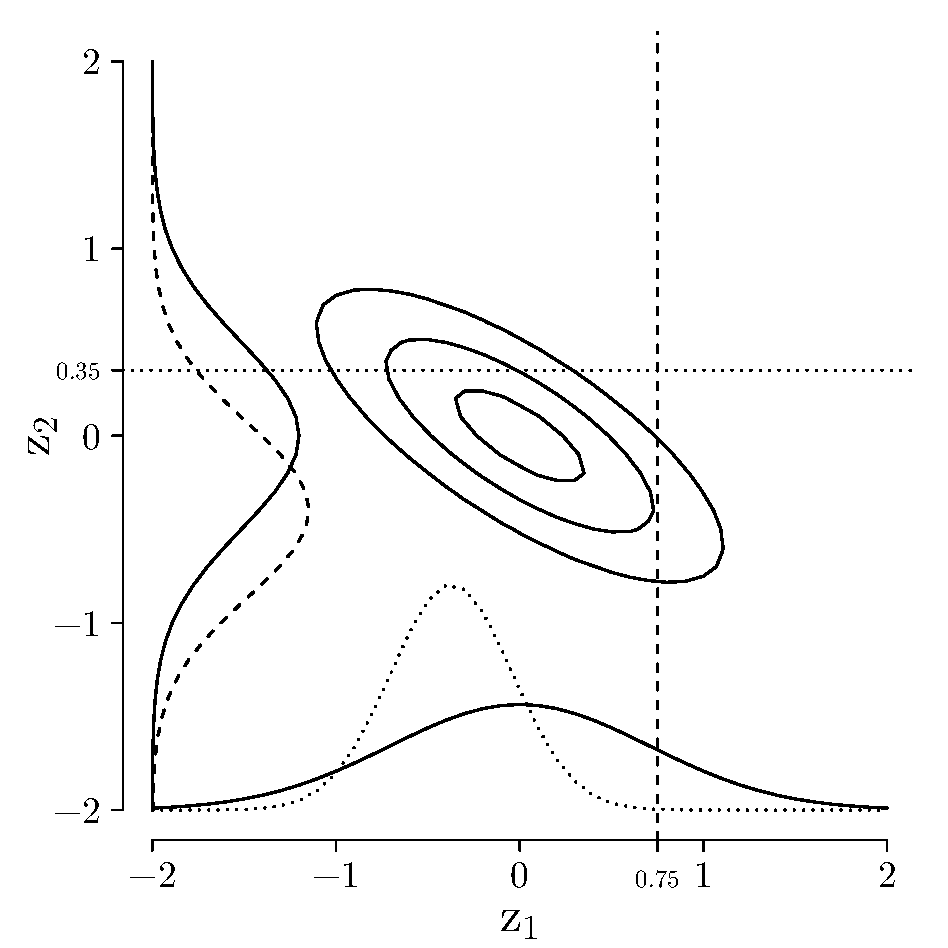
\includegraphics[scale=0.50]{../figures/chapter4/figures/plotBivariateNormal.pdf}
	\caption[Illustration of a bivariate Gaussian distribution]{An illustration of bivariate Gaussian distribution of random vector $Z = [Z_1, Z_2]$ having marginal means of $0.0$ and variances of $0.5$ and $0.25$, respectively and with covariance of $-0.265165$. The solid ellipsoids indicate the contour of joint density of random vector $[Z_1, Z_2]$. The two solid curves at the $x$- and $y$-axes indicate the marginal densities of $Z_1$ and $Z_2$, respectively. The dotted curve shows the conditional density of random variable $Z_1$ given $z_2 = 0.35$, while the dashed curve shows the conditional density of $Z_2$ given $z_1 = 0.75$.}
	\label{fig:plot_bivariate_normal}
\end{figure}

The joint density for Gaussian random vector is given in Eq.~(\ref{eq:gaussian_joint_density}.
\marginpar{joint density, illustrated}
For the bivariate random variable in the example, the density can be shown as contour plot in Fig.~\ref{fig:plot_bivariate_normal}.
In the figure, the solid ellipsoids are the iso-contours of the distribution, where each pair of values lies along the contour line has the same probability density value.

The two marginal densities for the example are shown as the solid curves plotted in the $x$ and $y$-axes, respectively.
\marginpar{marginal density, illustrated}
As illustrated, the marginalization of the joint distribution can be thought as a \emph{projection} of the $2$-dimensional distribution into each of the corresponding dimension.

Finally, two conditional distributions $p(z_1|z_2=0.35)$ and $p(z_2|z_1=0.75)$ are given as examples of conditioning a probability distribution in Fig.~\ref{fig:plot_bivariate_normal}.
\marginpar{conditional density, illustrated}
They are shown as dotted and dashed curves plotted in both axes.
Instead of projection to either of the axes, conditioning can be thought of as \emph{slicing} the $2$-dimensional distribution.
Conditioning two correlated random variables on one, in general, changes the shape of the distribution of the other variable.
From the figure, conditioning shifts the mean and reduces the variance of the resulting conditional distribution. 

% Drawing from Multivariate Gaussian
There are multiple ways to draw samples from a multivariate Gaussian distribution.
One method is particular require the deco
This method, so-called \emph{Cholesky} method, is detailed in Appendix.
A random number generator for the standard univariate distribution itself is widely available in many standard numerical computing environments.
The method in Appendix is used to generate 250 samples for the bivariate.
The resulting scatter plot and sample histograms of the marginal distributions 

% From Multivariate to Infinite Variate
\gls[hyper=false]{gp} can often be thought simply as a generalization of finite multivariate Gaussian random variable into an infinite multivariate one.
\marginpar{An entry to Gaussian Process}
To illustrate this idea, the marginal and conditional distributions of the bivariate distribution depicted in Fig.~ is plotted with the random variables at the same axis ($x$) while the range pf values of the variables are plotted in another axis ($y$).
The left panels shows the marginal distributions of random variables $Z_1$ and $Z_2$, where in Fig.~ they are plotted as black curves in their respective axes.
The center panel shows an observed value of $z_1 = 0.75$ depicted in Fig.~ as vertical dashed line.
Finally the right panel shows the conditional distribution of the non-observed variable $Z_2$ given $z_1 = 0.75$, which in Fig.~ was depicted as the dashed curve in the $y$-axis.
As it can be seen, the mean and standard deviation of the conditional distribution of $Z_2$ have been shifted and reduced, respectively, according to the information about $Z_1$.

Depiction in Fig.~ can easily be extended to a larger number of random variables, provided a valid mean vector and a valid covariance matrix.
Fig.~ shows such an extension to $15$-variate Gaussian random variable.
The origin of the underlying $15 \times 15$ covariance matrix is at the moment unimportant, but what the matrix does is defining how the variables are correlated to each other.
The whole covariance matrix, except its diagonal elements, is irrelevant in describing the marginal (Fig, left),
but it is significant in describing the shape of the conditional (Fig, right) according to Eqs.~.
As before, the conditional probability of the non-observed random variables are shifted and their standard deviation are reduced due to the information provided from the observed variables.

% Closing Sentence
Gaussian stochastic generalizes this procedure beyond $2$- or $15$-variate Gaussian random variable to an arbitrary number of variables at arbitrary locations in the real line.
It is easy to imagine that the shape of both marginals and conditionals will become smoother and smoother with increasing number of random variables in the $x$-axis, thus resembling more of a smooth function.
In fact, it is one of the interpretations of Gaussian process: a distribution over functions (citation). 

\subsection{Gaussian Process}

% What is a stochastic process
Gaussian stochastic process is a particular class of \emph{stochastic} or \emph{random process}.
\marginpar{Stochastic process}
Stochastic process is a collection of random variables, each of which are often indexed with certain underlying rules or ordering.
To be precise, a stochastic process is a set of random variables $\mathbf{Y} = \{Y_i, i \in I\}$, where $I$ is an index set, 
and it is defined on a probability space $(\Omega, \mathcal{F}, \mathbb{P})$, 
where $\Omega$, $\mathcal{F}$, and $\mathbb{P}$ are the sample space, the set of events, and the assigned probability to the event, respectively \cite{Syski2014}.

% Examples of stochastic process applications
For example, a time series can be modeled using stochastic process where the random variables are the observations taken at different time ordered sequentially.
\marginpar{Stochastic process applications}
In this case the index set is the time index of the observations.
A spatial model, as another example, can be modeled as a collection of random variables indexed by their locations in space.
And finally, in the metamodeling application, the random variables are collection of computational model output values at different input values.

% Gaussian stochastic process
\emph{Gaussian stochastic process} (GP, or Gaussian Random Field GRF) is defined as a collection of random variables, 
\emph{arbitrary number of which is a multivariate Gaussian random variable} \cite{Rasmussen2006, Debicki2014}.
\marginpar{Gaussian process}
To establish the connection with the notion of \emph{random function}, the collection of the above random variables refers to the collection of values of a random function $Y(\circ)$ at various possible input $\mathbf{x}$ in the domain $\mathcal{X} \subseteq \mathbb{R}^D$.
Specifically, $Y(\mathbf{x}), \, \text{for} \, \mathbf{x} \in \mathcal{X} \subseteq \mathbb{R}^D$ is a \emph{Gaussian process} if and only if for any choice from the finite set of input $\{\mathbf{x}_1, \mathbf{x}_2, \cdots, \mathbf{x}_L ; \, L \geq 1\}$, the random vector $\left[Y(\mathbf{x}_1), Y(\mathbf{x}_2), \cdots, Y(\mathbf{x}_L)\right]$ is a multivariate Gaussian random variable \cite{Santner2003}.

% Basic notation
A \gls[hyper=false]{gp} is fully specified by its mean and covariance functions, instead mean vector and covariance matrix.
A \gls[hyper=false]{gp} $Y$ on $\mathcal{X} \subseteq \mathbb{R}^D$ with a given mean function $m$ and covariance $K$ is denoted as
\begin{equation}
	Y(\mathbf{x}) \sim \mathcal{GP} \left(m(\mathbf{x}), K(\mathbf{x}, \mathbf{x}^*) \right)
\label{eq:gp_notation}
\end{equation}

% Mean Function
The mean function of a Gaussian process $Y(\mathbf{x})$ is the function $m: \chi \subseteq \mathbb{R}^D \mapsto \mathbb{R}$ defined as,
\marginpar{Mean function}
\begin{equation}
	m(\mathbf{x}) = \mathbb{E}[Y(\mathbf{x})]
\label{eq:gp_mean_functions}
\end{equation}

% Covariance Function
The covariance function of a Gaussian process $Y(\mathbf{x})$, on the other hand, is the function $K: (\chi \subseteq \mathbb{R}^D) \times (\chi \subseteq \mathbb{R}^D) \mapsto \mathbb{R}$ defined as,
\marginpar{Covariance Function}
\begin{equation}
	K(\mathbf{x}_i, \mathbf{x}_j) = \text{Cov}[Y(\mathbf{x}_i), Y(\mathbf{x}_j)]
\label{eq:gp_cov_functions}
\end{equation}
Notice that while the covariance function describes the covariance describes the covariance between pair of random function values, 
it is defined only as a function of the two inputs differentiating them.
Covariance function is also sometimes referred to as the \emph{covariance kernel} function as it defines the elements of the covariance matrix (see example below).
As such, not all functions of the pair of inputs $\mathbf{x}_i, \mathbf{x}_j$ are a \emph{valid} covariance function, but only the ones that yield a valid variance-covariance matrix given by condition in Eq.~(\ref{eq:covariance_matrix}). 

% Process Variance
Finally, the process variance is defined as the covariance between two random function values at the same input,
\marginpar{Process variance}
\begin{equation}
	K(\mathbf{x}_i, \mathbf{x}_i) = \text{Cov}[Y(\mathbf{x}_i), Y(\mathbf{x}_i)] = \mathbf{V}[Y(\mathbf{x}_i)]
\label{eq:process_variance}
\end{equation}

% Gaussian Stochastic Process and Multivariate Gaussian Random Variable
For a given finite $L$, a \gls[hyper=false]{gp} is reduced to a multivariate Gaussian random variable characterized by its mean vector $\boldsymbol{\mu}$ and covariance matrix $\boldsymbol{\Sigma}$,
\begin{equation}
	\begin{split}
		& [Y(\mathbf{x}_i)] \sim \mathcal{N}(\boldsymbol{\mu}, \boldsymbol{\Sigma}) \quad ; \, i = 1, 2, \cdots, L \\
		& \boldsymbol{\mu} = [m(\mathbf{x}_1), m(\mathbf{x}_2), \cdots, (\mathbf{x}_L)]^T \\
		  & \boldsymbol{\Sigma} = 
				\begin{pmatrix}
					\mathbf{V}[Y(\mathbf{x}_1)]  & \cdots & \text{Cov}[Y(\mathbf{x}_1), Y(\mathbf{x}_L)]\\
					\vdots	& \ddots & \vdots\\
					\text{Cov}[Y(\mathbf{x}_L), Y(\mathbf{x}_1)]  & \cdots  & \mathbf{V}[Y(\mathbf{x}_L)]\\
			\end{pmatrix} \\
	\end{split}
\label{eq:gp_to_mvn}
\end{equation}

% Example, introduced
The shape of the random function drawn from a \gls[hyper=false]{gp} is characterized by its mean and covariance functions.
Brief explanations of these functions will be provided in the next two subsections.
\marginpar{fully specified GP, an example}
In the meantime, an example of a fully specified Gaussian process will be used to illustrate how samples of functions can be drawn from such a stochastic process.
For the example, the following mean and covariance function will be used
\begin{equation}
	\begin{split}
		m(\mathbf{x}) & = 0 \\
		K(\mathbf{x}, \mathbf{x}^*) & = \sigma^2 \exp{\left[-\frac{(\mathbf{x} - \mathbf{x}^*)^2}{2\theta^2}\right]} = 10 \exp{\left[-\frac{(\mathbf{x} - \mathbf{x}^*)^2}{0.98}\right]}
	\end{split}
\label{eq:gp_example}
\end{equation}
where $x$ is a $1$-dimensional input parameter such that $x \in [-2, 2]$.
The mean function is set to constant zero, while the covariance function is chosen to be the so-called \emph{Gaussian covariance function} (which will be detailed in the sequel).
The Gaussian covariance function is parameterized by the characteristic length scale $\theta$ which is set to $0.70$.
This parameter is often referred to as the \emph{hyper-parameter} of the function.
Finally, $\sigma^2$ is the common variance of the stochastic process and it is set to $10$.

% Example continued, sample path
To generate random draws of function from the fully specified \gls[hyper=false]{gp} given in Eq.~(\ref{eq:gp_example}), 
first it must be specified at which input $x$ the function values are to be drawn.
\marginpar{sample path (trajectory) of a GP}
For the present example, $x$ is chosen to be uniformly distributed $\{-2 + 0.2 \times i\}_{i=0}^{20}$.
By specifying these locations, the $21$-variates Gaussian random variable can be constructed using Eq.~(\ref{eq:gp_to_mvn}) with the elements of variance-covariance matrix computed by the formula in Eq.~(\ref{eq:gp_example}) for all pairs of inputs.
Examples of $5$ realizations from the \gls[hyper=false]{gp} are shown in the left panel Fig~\ref{fig:sample_path_unconditional}.
A realization of a \gls[hyper=false]{gp} on a select input locations is also called a \emph{trajectory} or a \emph{sample path} of the process \cite{Santner2003}.
In this thesis the term \emph{sample path} will be used interchangeable with the term realization of a \gls[hyper=false]{gp}.
\normdoublefigure[pos=tbhp,
                  mainlabel={fig:sample_paths},
                  maincaption={Five realizations (sample paths) of a Gaussian process specified in Eq.~(\ref{eq:gp_example}) at $x_i = \{-2 + 0.2 \times i\}_{i=0}^{20}$. Shaded area indicates the area enveloped by twice standard deviation of the process (or $95\%$ probability region). In the right panel, the sample paths are drawn conditional on $6$ observed values (cross symbols).},%
                  leftopt={width=0.45\textwidth},%width=0.45\textwidth},
                  leftlabel={fig:sample_path_unconditional},
                  leftcaption={Unconditional},
                  %leftshortcaption={},%
                  rightopt={width=0.45\textwidth},%width=0.45\textwidth},
                  rightlabel={fig:sample_path_conditional},
                  rightcaption={Conditional},
                  %rightshortcaption={},
                  %spacing={\hfill}
                 ]
{../figures/chapter4/figures/plotSamplePath.pdf}
{../figures/chapter4/figures/plotSamplePathCond.pdf}

% Example, conditional simulation
Suppose now that values of $6$ variables are fully observed as follows $\{(x_i, y_i)\}_{i=1}^{6} = \{(-2.0, -0.75), (-1.2, 1.5), (-0.8, 2.75), (0.4, 3.75),$ 
$(1.2, -1.3), (1.8, -3.8)\}$.
\marginpar{conditional sample path}
The conditional $15$-variates Gaussian distribution can be constructed in the same manner as before with the conditional mean and covariance following Eqs.~.
Examples of $5$ sample paths from such conditional distribution are shown in Fig.~\ref{fig:sample_path_conditional}.
Observe that the standard deviations of the observed variables are zero and the areas between known values are substantially reduced.

% Strongly Stationary
An assumption for a class of stochastic process commonly made for convenience is \emph{stationarity}.
\marginpar{strongly stationary process}
A stochastic process $Y(\circ)$ is called \emph{strictly/strongly stationary} if and only if for any finite set of inputs $\{\mathbf{x}_1, \mathbf{x}_2,$
$\cdots, \mathbf{x}_L\} \in \mathcal{X} \subseteq \mathbb{R}^D$ with $L \leq 1$, 
and for $\mathbf{h} \in \mathbb{R}^D$ such that $\{(\mathbf{x}_1 + \mathbf{h}),$ 
$(\mathbf{x}_2 + \mathbf{h}), \cdots, (\mathbf{x}_L + \mathbf{h})\} \in \mathcal{X}$, the distribution of random vector $[Y(\mathbf{x}_1 + \mathbf{h}), $
$Y(\mathbf{x}_2 + \mathbf{h}), \cdots, Y(\mathbf{x}_L + \mathbf{h})]$ is \emph{the same as} the distribution of random vector $[Y(\mathbf{x}_1 + \mathbf{h}), Y(\mathbf{x}_2 + \mathbf{h}), \cdots, Y(\mathbf{x}_L + \mathbf{h})]$ \cite{Santner2003, Bachoc2013}.
In other words, the process is invariant under translation.

% Weakly Stationary
The \emph{weakly stationary process} used stronger assumption than the strongly stationary process.
\marginpar{weakly stationary process}
A stochastic process $Y(\circ)$ is called \emph{weakly stationary} if and only if
the first two moments of the process are constant.
As such, the weakly stationary process is also referred to as \emph{second-order stationary process}.

% Stationary, Isotropic Covariance Function
As mentioned, a \gls[hyper=false]{gp} is fully defined by its mean and covariance functions.
\marginpar{stationary, isotropic covariance function}
Therefore, if two \glspl[hyper=false]{gp} have the same mean and covariance functions defined over the same domain then the two process have exactly the same same distribution and are the same process.
Furthermore, for the case of \gls[hyper=false]{gp}, the notions of strongly stationary and weakly stationary coincide.
This implies that a stationary \gls[hyper=false]{gp} has a constant mean and a constant variance, as well as a covariance function that satisfies the condition of being invariant under translation as follows,
\begin{equation}
	\text{Cov}[Y(\mathbf{x}_i), Y(\mathbf{x}_j)] = \text{Cov}[Y(\mathbf{x}_i + \mathbf{h}), Y(\mathbf{x}_j + \mathbf{h})] = K (\mathbf{x}_i - \mathbf{x}_j)
\label{eq:stationary_covariance}
\end{equation}
In stationary \gls[hyper=false]{gp}, the covariance of random function values between two input points is only determined by the \emph{distance} between the two inputs and the covariance function is called \emph{stationary, isotropic covariance function} \cite{Rasmussen2006}. 
The notion of distance used in the above definition depends on the specific type of the covariance function as will be explained in the next subsection.
Additionally, following Eq.~\ref{eq:stationary_covariance}, the process variance can be defined as the covariance at zero distance or $K(0)$, which is constant across input parameter space.

% Non-Stationary Gaussian Process
A more flexible class of \gls[hyper=false]{gp} models can be constructed by relaxing the stationarity assumption.
\marginpar{non-stationary process}
However, stationarity is often assumed because it requires less assumption than the alternatives, considered non-informative, and therefore more generic \cite{Currin1991}.
Moreover, the stationary process remains important to study as they serve as building block for more advanced models \cite{Santner2003}.
For instance, the stationarity assumption can be relaxed simply by considering non-constant mean function as proposed in  \cite{Marrel2008,Ginsbourger2009}, while keeping the covariance part stationary.
Another alternative is to consider multiple stationary covariance functions defined for each partitioned region of the whole input parameter space as proposed in \cite{Gramacy2008}.

\subsection{Covariance Kernel Function}\label{sub:gp_covariance}

Covariance kernel function determines the covariation structure of dependent data.
This, in turn, determines the behavior (or shape) of the sample path of the outputs between input points.
For a stationary covariance function, it is more convenient to separate the constant stochastic process variance $\sigma^2$ and the stochastic process kernel correlation function $R(\circ,\circ)$ between two input points using the following relation,
\begin{equation}
	K (\mathbf{x}_i, \mathbf{x}_j) = \sigma^2 R(\mathbf{x}_i, \mathbf{x}_j) 
	\label{eq:cov_function}
\end{equation}
where $R$, the correlation kernel function, is defined such that $\forall \, \mathbf{x}_i, \mathbf{x}_j \in \chi \subseteq \mathbb{R}^D$;
and $\sigma^2$ is the aforementioned stochastic process variance, which determines the scale of variation magnitude of the output space.

In the following, three different types of stationary correlation kernel functions are presented. 
These functions, namely \emph{Gaussian}, \emph{power-exponential}, and \emph{Mat\'ern class} kernels are widely applied in the simulation metamodeling literature.
\marginpar{one-dimensional correlation kernel, $r$}
For each, the function is defined and several sample paths are drawn to illustrate the effect of different kernels and different respective parameters on the realization.
At first, only $1$-dimensional kernel functions denoted by $r(x_i, x_j)$ are described.
Afterward, these $1$-dimensional functions are used to create a multidimensional kernel function $R(\mathbf{x}_i, \mathbf{x}_j)$ by means of tensor product.

\subsubsection{Gaussian Kernel}\label{subsub:gp_gaussian_cov}

The Gaussian correlation kernel function, also known as the \emph{squared exponential} kernel, is given by the following formula \cite{Roustant2012,Santner2003,Rasmussen2006},
\begin{equation}
	r(x_i, x_j; \theta) = \exp{\left[- \frac{(x_i - x_j)^2}{2 \theta^2}\right]}
\label{eq:gaussian_kernel}
\end{equation}

The Gaussian kernel is parameterized by only a single \emph{hyper-parameter} $\theta$ that defines the characteristic length-scale of the process (or simply \emph{the scale parameter}).
\marginpar{characteristic length-scale parameter}
Fig.~\ref{fig:plot_corrfun_gauss} shows the correlation value as function of Euclidian distance, $(x_i - x_j)^2$, between input points according to the Gaussian kernel, 
for 3 different characteristic length scales.
Obviously, for smaller $\theta$ the correlation between two inputs drops more quickly over shorter distance, and vice versa.
\begin{figure}[bth]
	\centering
	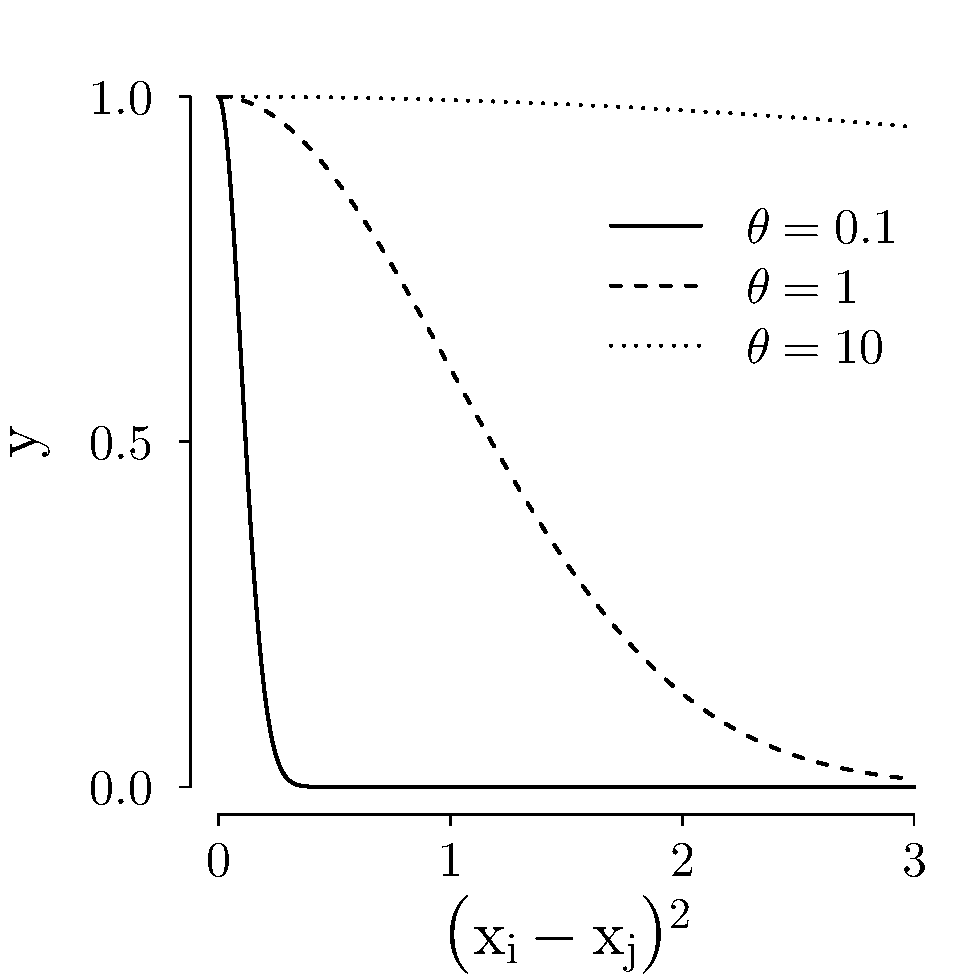
\includegraphics[scale=0.35]{../figures/chapter4/figures/plotCorrFunGauss.pdf}
	\caption[Gaussian correlation kernels with 3 different characteristic length scales]{Examples of Gaussian correlation kernels with 3 different characteristic length scales}
	\label{fig:plot_corrfun_gauss}
\end{figure}

The characteristic length-scale of a Gaussian kernel determines the range over which the distance between two input locations affects the output correlation.
To be precise, the notion how similar (or dissimilar) two input locations is defined relative to the characteristic length-scale.
With a very short length-scale, the output of random functions becomes easily uncorrelated except for a very close (similar) inputs.
The realization of the process, therefore, will exhibit more erratic behavior in short length scale as it allows for more abrupt changes over shorter distance and less dependent of the neighboring values.
On the other hand, with a longer length-scale, the output of random function tends to be highly correlated except for very different input values and thus the realization will exhibit more rigid pattern.
Gaussian kernel, however, always produces smooth realization. That is, two input points that have a zero separation on the limit are both continuous and differentiable 
(see the neighborhood of the origin of Fig.~\ref{fig:plot_corrfun_gauss}).
The Gaussian kernel is widely applied in the metamodeling literature and almost become a default choice for the correlation kernel \cite{Kennedy2006},
though as mentioned in \cite{Rasmussen2006} the overly smooth process can result in either physically unrealistic or numerically difficult situations (i.e., the resulting variance-covariance matrix is ill-conditioned for poorly select design points).

Fig.~\ref{fig:plot_corrfun_gauss_realizations} shows a comparison between realizations of a \gls[hyper=false]{gp} using Gaussian kernel for three different characteristic length-scales.
The short length scale, illustrated on the left panel, allows for more sudden change in the output values while the long length scale on the right shows smoother (and rigid) pattern for the same input domain ($0.0 \leq x \leq 3.0$). 
Also notice that the realizations with the shorter length scale produces more local maxima and minima.
\bigtriplefigure[pos=tbhp,
								 mainlabel={fig:plot_corrfun_gauss_realizations},
			           maincaption={Examples of realizations from \gls[hyper=false]{gp} with Gaussian correlation kernel for $3$ different values of characteristic length-scale. The plotting range of the $y$-axis for each panel are set to $\pm \, 3 \times \sigma$. Each process has the same process variance, $\sigma^2 = 1.0$},
			           mainshortcaption={Realizations of random function drawn from \gls[hyper=false]{gp} with Gaussian kernel},%
			           leftopt={width=0.30\textwidth},
			           leftlabel={fig:plot_corrfun_gauss_realization_1},
			           leftcaption={},
			           midopt={width=0.30\textwidth},
			           midlabel={fig:plot_corrfun_gauss_realization_2},
			           midcaption={},
			           rightopt={width=0.30\textwidth},
			           rightlabel={fig:plot_corrfun_gauss_realization_3},
			           rightcaption={},
			           spacing={},
			           spacingtwo={}]
{../figures/chapter4/figures/plotCorrFunGaussRealization_1}
{../figures/chapter4/figures/plotCorrFunGaussRealization_2}
{../figures/chapter4/figures/plotCorrFunGaussRealization_3}

\subsubsection{Power-Exponential Kernel}

The Gaussian correlation kernel belongs to a wider class of $2$-parameter kernel function family called the \emph{power-exponential} kernel and is given by \cite{Roustant2012,Santner2003,Rasmussen2006},
\begin{equation}
	r(x_i, x_j; \theta, p) = \exp{\left[ - \left( \frac{|x_i - x_j|}{\theta} \right)^p \right]} \, \text{for} \, \theta > 0.0 \, \text{and} \, 0 < p \leq 2
\label{eq:powexp_kernel}
\end{equation}

The parameter $\theta$ remains the (length-) scale parameter of the process, while the additional parameter $p$ is referred to as the shape parameter of the process.
\marginpar{shape parameter}
Specifically, the shape parameter $p$ determines the differentiability of the process at the origin (citation needed).
Fig.~\ref{fig:plot_corrfun_powexp} shows the correlation value of power-exponential kernel with three different values of $p$ and $\theta$ as function of $L_1$ norm.
\bigtriplefigure[pos=tbhp,
								 mainlabel={fig:plot_corrfun_powexp},
			           maincaption={Examples of power exponential kernel functions for different values of shape parameter $p$ and scale parameter $\theta$ as function of $L_1$ norm.},
			           mainshortcaption={Examples of power exponential kernel functions},%
			           leftopt={width=0.30\textwidth},
			           leftlabel={fig:plot_corrfun_powexp_1},
			           leftcaption={},
			           midopt={width=0.30\textwidth},
			           midlabel={fig:plot_corrfun_powexp_2},
			           midcaption={},
			           rightopt={width=0.30\textwidth},
			           rightlabel={fig:plot_corrfun_powexp_3},
			           rightcaption={},
			           spacing={},
			           spacingtwo={}]
{../figures/chapter4/figures/plotCorrFunPowExp_1}
{../figures/chapter4/figures/plotCorrFunPowExp_2}
{../figures/chapter4/figures/plotCorrFunPowExp_3}

Although, strictly speaking, only when $p = 2$ that the power-exponential correlation is differentiable at the origin (thus guarantee the smoothness of the realization),
the shape parameter does dictate the apparent roughness of the sample path drawn from the process as illustrated in Fig.~\ref{fig:plot_corrfun_gauss_realizations} \cite{Rasmussen2006}.
\bigtriplefigure[pos=tbhp,
								 mainlabel={fig:plot_corrfun_powexp_realizations},
			           maincaption={Several realizations from \gls[hyper=false]{gp} with power-exponential kernel functions of different shape $p$ and scale $\theta$ parameters.},
			           mainshortcaption={Examples of power exponential kernel functions},%
			           leftopt={width=0.30\textwidth},
			           leftlabel={fig:plot_corrfun_powexp_realization_1},
			           leftcaption={},
			           midopt={width=0.30\textwidth},
			           midlabel={fig:plot_corrfun_powexp_realization_2},
			           midcaption={},
			           rightopt={width=0.30\textwidth},
			           rightlabel={fig:plot_corrfun_powexp_realization_3},
			           rightcaption={},
			           spacing={},
			           spacingtwo={}]
{../figures/chapter4/figures/plotCorrFunPowExpRealizations_1}
{../figures/chapter4/figures/plotCorrFunPowExpRealizations_2}
{../figures/chapter4/figures/plotCorrFunPowExpRealizations_3}

It is argued in \cite{Marrel2008} that the power-exponential kernel function is an appropriate choice in metamodeling application due to its flexibility of representing different shape with respective to its regularity and differentiability mainly controlled through the additional parameter $p$.
\marginpar{exponential kernel}
For instance, Gaussian correlation kernel is a special case of the power-exponential kernel when $p$ equals to 2. 
Another special case is when $p = 1$ which is called the \emph{exponential} kernel.
In this particular case, realizations of which are depicted in Fig.~\ref{fig:plot_corrfun_powexp_realization_2}, the process is continuous but not differentiable \cite{Rasmussen2006}.

\subsubsection{Mat\'ern Class Kernel}

The Mat\'ern class correlation kernel is another $2$-parameter kernel family and it is given by the following formula
\lipsum[2]

\subsection{Multidimensional Construction}

In order to create a valid multidimensional correlation kernel function from a valid $1$-dimensional correlation function given above, 
a tensor product construction is used as follows,
\marginpar{tensor product}
\begin{equation}
	R(\mathbf{x}_i, \mathbf{x}_j) = \prod_{d = 1}^{D} r_d \left(x_i^{(d)}, x_j^{(d)}\right)
\label{eq:tensor_product}
\end{equation}
where $r_d$ is a $1$-dimensional correlation kernel function for the $d$-th input dimension;
while $x_i^{(d)}$ and $x_j^{(d)}$ are a pair of values in the $d$-th input dimension.

Although it is possible to mix different types of correlation function or use different kind of multidimensional construction (see for example \cite{Higdon2002}),
the tensor product with the same correlation function for each input dimension is the most well-established 
and, by far, the most popular approach in the applied metamodeling literature to date \cite{Roustant2012,Sacks1989,Sacks1989a,Santner2003,Currin1991,Marrel2008,Bachoc2014,Kennedy2006,Jones2009}.

Fig.~\ref{fig:random_surfaces} shows two examples of realizations of random surface drawn from a multidimensional \gls[hyper=false]{gp} with the same process variance ($\sigma^2 = 10.0$) but with two different correlation kernels.
On the left is an example of a realization drawn from the \gls[hyper=false]{gp} using Gaussian correlation kernel function with relatively the characteristic length scale in $y$-direction is four times the scale in $x$-direction.
On the right is an example of a realization drawn from the \gls[hyper=false]{gp} using Mat\'ern correlation kernel function.
For this case, the shape parameter is three times larger in the $x$-direction than in the $y$-direction.
As such, for both cases, the surface appears less smooth in one of the direction.
\bigdoublefigure[pos=tbhp,
                 mainlabel={fig:random_surfaces},
								 mainshortcaption={Random surface realizations},
                 maincaption={Two random surfaces drawn from two different multidimensional \gls[hyper=false]{gp} with the same process variance of $\sigma^2 = 9.0$. Differences in the scale (for Gaussian) and shape (for Mat\'ern) parameters for the inputs yield smoother path in one direction. The color scheme is the same for both plots with the range of $\pm \, 3 \times \sigma$.},
                 leftopt={width=0.475\textwidth},
                 leftlabel={fig:random_surface_gaussian},
                 leftcaption={Gaussian, $\theta_x = 0.5, \theta_y = 2.0$},
                 rightopt={width=0.475\textwidth},
                 rightlabel={fig:random_surface_matern},
                 rightcaption={Mat\'ern, $\theta_x = 1.5, \theta_y = 0.5$},
                 ]
{../figures/chapter4/figures/plotRandomSurface_1}
{../figures/chapter4/figures/plotRandomSurface_2}

\subsection{Process Variance}

For stationary \gls[hyper=false]{gp}, the shape of sample path is determined solely by the form of the correlation.
The role of process variance according to Eq.~(\ref{eq:cov_function}) is to determine the scale of magnitude of output variation. 
Fig.~\ref{fig:plot_process_variance} gives an illustration of realizations drawn from a set of \glspl[hyper=false]{gp} with the same kernel correlation function (i.e., Gaussian kernel with $\theta = 1.0$), 
but with different values of process variance.
As it can be seen, the visible features of the realizations remain the very similar to each other.
What has changed, however, is the scale of the variation in the output space.  
\bigtriplefigure[pos=tbhp,
								 mainlabel={fig:plot_process_variance},
			           maincaption={Realizations of \gls[hyper=false]{gp} with Gaussian correlation kernel for $3$ different values of process variance. The plotting range of the $y$-axis for each panel are set to $\pm \, 3 \times \sigma$.},
			           mainshortcaption={Effect of different process variance values on GP realization},%
			           leftopt={width=0.30\textwidth},
			           leftlabel={fig:plot_process_variance_1},
			           leftcaption={},
			           midopt={width=0.30\textwidth},
			           midlabel={fig:plot_process_variance_2},
			           midcaption={},
			           rightopt={width=0.30\textwidth},
			           rightlabel={fig:plot_process_variance_3},
			           rightcaption={},
			           spacing={},
			           spacingtwo={}]
{../figures/chapter4/figures/plotProcessVariance_1}
{../figures/chapter4/figures/plotProcessVariance_2}
{../figures/chapter4/figures/plotProcessVariance_3}

\subsection{Mean Function}
%**************************************************************
\section{Gaussian Process Metamodel}\label{sec:gp_metamodeling}
%**************************************************************

% Kriging Model, Drift and Bias
To formalize the use of in the meta-modeling of computer simulation, 
consider once again a computer code represented as 

The output of code at an arbitrary inputs, $\mathbf{x_o}$, is then modeled using a predictor of the following form
\begin{equation}
	Y (\mathbf{x_o}) = \mu (\mathbf{x_o}) + Z (\mathbf{x_o})
\label{eq:kriging_model}
\end{equation}
The equation above, also known as the \emph{Kriging} model (cite Owen, Simpson, Dupuy)\footnote{in fact, the term Kriging model will be used interchangeably as Gaussian process metamodel in this thesis} , consists of two components:
\begin{itemize}
	\item The \emph{mean/drift/trend} term, a deterministic function
	\begin{equation}
		\mu: \mathbf{x} \in \mathcal{X} \subseteq \mathbb{R}^D \mapsto \mathbb{R}
	\label{eq:trend_function_mapping}
	\end{equation}
	The trend term, in turn, usually consists of general linear model of polynomials (cite Owen and Dupuy, Marrel).
	\begin{equation}
		\mu(\mathbf{x}) = \sum_{j=0}^{k} \beta_j h_j(\mathbf{x})
	\label{eq:trend_function_definition}
	\end{equation}
	The trend term captures the global input output space which has an equivalent interpretation to that of a linear regression model\footnote{$Y() = \mu(\mathbf{x} + \epsilon$ with $\epsilon$ is Normally independent and identically distributed measurement error term}.
	\item The \emph{bias} term, a stochastic process. 
	This term, in turn, usually modeled using zero mean, stationary Gaussian stochastic process (such as presented in Section~\ref{sub:gp_covariance}).
	\begin{equation}
		\mathcal{Z}(\mathbf{x}) \sim \mathcal{GP}(0, R(\mathbf{x},\mathbf{x}^*))
	\label{eq:stationary_gp}
	\end{equation}
	The bias term captures the local variation of the output space such that it pulls the predictor.
	The term local here is referring to the neighborhood of training data.
	In linear regression model the error between observation and prediction is due to experimental error.
	This, in essence, what distinguishes kriging model to ordinary least square.
	Furthermore, by using stationary Gaussian process it is also assumed that the bias term will be a function of distance between design points and test point. 
\end{itemize}

% Hyper-parameters
Additionally, according to the above formulation, a \gls[hyper=false]{gp} metamodel contains several parameters called the \emph{hyper-parameters}.
\marginpar{hyper-parameters}
This term is used to distinguish them from the parameter associated with the original simulation model which is referred to as the model parameter or often simply as the parameter.
The hyper-parameters of a \gls[hyper=false]{gp} metamodel are the ones associated with the chosen trend function (Eq.~\ref{eq:trend_function_definition});
the ones associated with select correlation functions (Section~\ref{sub:gp_covariance}); and the one associated with the process variance $\sigma^2$.
The total number of hyper-parameters depends on the number of simulation model parameters as well as the select structure of mean and correlation functions.
For instance, for a $D$-parameter simulation model represented using \gls[hyper=false]{gp} metamodel with a constant mean and Gaussian correlation functions (Eq.~(\ref{eq:gaussian_kernel})), 
the total number of hyper-parameters $\boldsymbol{\Psi} = (\mu, \sigma^2, \boldsymbol{\theta})$ is $D + 2$.
On the other hand, the same model represented using a \gls[hyper=false]{gp} metamodel with linear first-order mean and power-exponential functions (Eq.~(\ref{eq:powexp_kernel})),
the total number of the hyper-para\-meters $\boldsymbol{\Psi} = (\boldsymbol{\beta}, \sigma^2, \boldsymbol{\theta}, \mathbf{p})$ is $3D + 2$.

% Three classes of Kriging Model
Two classes of Kriging models can be distinguished depending on what is known about the hyper-parameters: 
\emph{Simple Kriging} and \emph{Universal Kriging}.

\subsection{Simple Kriging}\label{sub:gp_sk}

% Simple Kriging
Simple Kriging is the simplest case of the Kriging models where all the hyper-parameters involved are assumed to be known.
\marginpar{simple Kriging}
In that case the estimation of code output at an arbitrary input location becomes straightforward.
Following the formulation above, 
a \gls[hyper=false]{gp} metamodel, then by definition implies that the computer code outputs at every input locations are jointly Gaussian.
As such, the code outputs at the training inputs $\mathbf{DM} = \{\mathbf{x}_i\}_{i=1}^N, Y(\mathbf{DM}) = (Y(\mathbf{x}_1), Y(\mathbf{x}_2), \cdots, Y(\mathbf{x}_N))$
and the output at an arbitrary input $\mathbf{x}_o$, $Y(\mathbf{x}_o)$ are distributed jointly as an $N+1$-dimensional Gaussian,
\begin{equation}
	\begin{bmatrix}
			Y(\mathbf{DM}) \\
			Y(\mathbf{x}_o)
		\end{bmatrix} \sim \mathcal{N} \left(
			\begin{bmatrix}
				\mu(\mathbf{DM}) \\
				\mu(\mathbf{x}_o)
			\end{bmatrix}, \sigma^2
			\begin{bmatrix}
				R(\mathbf{DM}, \mathbf{DM})  & R(\mathbf{DM}, \mathbf{x}_o) \\
				R(\mathbf{x}_o, \mathbf{DM}) & R(\mathbf{x}_o, \mathbf{x}_o)
			\end{bmatrix} \right)
\label{eq:joint_training_test}
\end{equation}
where
\begin{itemize}
	\item $\mu(\mathbf{DM})$ is the vector of mean at the training points;
		\begin{equation}
			\mu(\mathbf{DM}) = (\mu(\mathbf{x}_1), \mu(\mathbf{x}_2), \cdots, \mu(\mathbf{x}_N)) 
		\label{eq:training_mean_vector}
		\end{equation}
	\item $\mu(\mathbf{x}_o)$ is the mean at an arbitrary test location;
	\item $R(\mathbf{DM}, \mathbf{DM})$ is the $N \times N$ correlation matrix between outputs at the training points
		\begin{equation}
			R(\mathbf{DM}, \mathbf{DM}) = 
				\begin{bmatrix}
					R(\mathbf{x}_1, \mathbf{x}_1) & \cdots												& R(\mathbf{x}_1, \mathbf{x}_N) \\
					\vdots												& \ddots												&	\vdots \\
					R(\mathbf{x}_N, \mathbf{x}_1)	&	R(\mathbf{x}_N, \mathbf{x}_2) & R(\mathbf{x}_N, \mathbf{x}_N)
				\end{bmatrix}
		\label{eq:training_correlation_matrix}
		\end{equation}
	\item $R(\mathbf{DM}, \mathbf{x}_o) = R(\mathbf{x}_o, \mathbf{DM})$ is the $N \times 1$ vector of correlation between outputs at the training points and the output at the test point
			\begin{equation}
				R(\mathbf{x}_o, \mathbf{DM}) = R(\mathbf{DM}, \mathbf{x}_o) =  
					\begin{bmatrix}
						R(\mathbf{x}_o, \mathbf{x}_1) \\
						\vdots												\\
						R(\mathbf{x}_o, \mathbf{x}_N)	
					\end{bmatrix}
			\label{eq:training_test_correlation}
			\end{equation}
		\item and $R(\mathbf{x}_o, \mathbf{x}_o)$ is the correlation of the output at the test input with itself. By definition this correlation is equal to $1$.
\end{itemize}

% Conditional Distribution, Simple Kriging
Provided that the outputs at the training inputs are fully observed (i.e., the code is actually run at those inputs),
then the output at the test input $Y(\mathbf{x}_o)$ \emph{given	} the observed outputs $Y(\mathbf{DM}) = \mathbf{y} = (y_1, y_2, \cdots,$ 
$y_N)^T$ is a conditional Gaussian random variable,
\begin{equation}
	Y(\mathbf{x}_o) | Y(\mathbf{DM}) = \{y_i\}_{i=1}^N \sim \mathcal{N} \left( m_{SK}(\mathbf{x}_o), s^2_{SK}(\mathbf{x})\right)
\label{eq:joint_training_test}
\end{equation}
where $\mu_{SK}$ and $s^2_{SK}$ are the mean and the variance of the distribution, respectively.
They are also often referred to as the \emph{simple Kriging mean} and \emph{simple Kriging variance}, respectively.

% Kriging Predictor, the mean
The simple Kriging mean (or the \emph{Kriging predictor}) is expressed as follow
\marginpar{(simple) Kriging mean}
\begin{equation}
	m_{SK} (\mathbf{x}_o) = \mu (\mathbf{x}_o) + R^T(\mathbf{x}_o, \mathbf{DM}) R^{-1}(\mathbf{DM}, \mathbf{DM}) (\mathbf{y} - \mu(\mathbf{DM}))
\label{eq:mean_sk}
\end{equation}
% Kriging Variance
The simple Kriging variance, on the other hand, is expressed as
\marginpar{(simple) Kriging variance}
\begin{equation}
	s^2_{SK} (\mathbf{x}_o) = \sigma^2 (1 - R^T(\mathbf{x}_o, \mathbf{DM}) R^T(\mathbf{DM}, \mathbf{DM}) R(\mathbf{x}_o, \mathbf{DM}))
\label{eq:variance_sk}
\end{equation}
The expressions for the mean and the variance above are obtained through the conditioning operation of the Gaussian random vector in Eq.(~\ref{eq:joint_training_test}) (See Appendix). 
In practice, the Kriging mean are used as a predictor of the code output at an arbitrary input location, 
while the variance is used as a measure of error of that prediction.

% Interesting Observation
The simple Kriging model has several interesting features:
\begin{itemize}
	% Linearity
	\item The Kriging predictor given by the mean in Eq.(\ref{eq:mean_sk}) is a \emph{linear predictor}. 
				\marginpar{linear predictor}
	      In other words, the centered predictor ($m_{SK}(\mathbf{x}_o) - \mu (\mathbf{x}_o)$)  is a weighted linear combination of the centered data 
	      ($\mathbf{y} - \mu(\mathbf{DM})$).
				The weights depends on the correlation function $R(\circ,\circ)$, the design of training points $\mathbf{DM}$, and the distance between the test point and the training points.
	% Interpolant
	\item The variance collapses at the training points, that is plugging-in $\mathbf{x}_i \in DM$ into Eq.(\ref{eq:variance_sk}) will yield $s^2_{SK}(\mathbf{x}_i) = 0$.
				\marginpar{Kriging as an interpolant}
	      As such, the Kriging predictor is also an \emph{interpolant}, which exactly fits the observed data (i.e., deterministic code output at the training inputs).
	% Dependence of the variance
	\item The variance on a given test point does not depend on the observed data.
				\marginpar{Variance as function of distance between test and training points}
	      Strictly speaking, it is only dependent on the process variance $\sigma^2$ and the correlation function $R(\circ,\circ)$.
				Furthermore, the variance on a given test point is also equal or less than the process variance, 
				the difference of which depends on the distance between $\mathbf{x}_o$ and the training points $\mathbf{DM}$.
				The closer $\mathbf{x}_o$ is to the training points, the smaller the variance at that point.
	% Epistemic Uncertainty interpretation
	\item Being the variance of a conditional Gaussian distribution, the Kriging variance can be intuitively interpreted as the posterior \emph{uncertainty} of the prediction given the observed data.
				\marginpar{Variance as measure of epistemic uncertainty}
	      The nature of this uncertainty is epistemic as, in the case of this thesis, the computer code that underlies the observed data is deterministic.
				In other words, the uncertainty associated with the prediction at an arbitrary input is due to the lack of knowledge because the code itself is not run at that point.
				However, the prediction at that point is informed by the observed data as contained in the training data.
\end{itemize}

\subsection{Universal Kriging and Hyper-Parameter Estimation}\label{sub:gp_uk}

% Ordinary and Universal Kriging
In most practical situation, however, the values of the hyper-parameters are not known a priori.
This is indeed the case for the Universal Kriging model where all the hyper-parameters values associated with both a linear mean and covariance functions are to be estimated simultaneously from the training data.


% Likelihood
To estimate the values of the hyper-parameters $\boldsymbol{\Psi}$ of a chosen structure of mean and covariance functions,
\marginpar{the likelihood function} 
it is should be first acknowledged that under \gls[hyper=false]{gp} model, the distribution of the observed data given a Gaussian process $\mathbf{y} \, | \, Y(\mathbf{x}), \boldsymbol{\Psi}$ is Gaussian such that
\begin{equation}
	\mathcal{L}(\boldsymbol{\Psi}; \mathbf{y}) = \frac{1}{(2\pi)^{N/2}(\sigma)^{N/2}|\mathbf{R}|^{1/2}} \exp{\left[- \frac{(\mathbf{y} - \mathbf{F} \boldsymbol{\beta})^T \mathbf{R}^{-1} (\mathbf{y} - \mathbf{F} \boldsymbol{\beta})}{2\sigma^2}\right]}
\label{eq:gp_likelihood}
\end{equation}
The term above is called the \emph{likelihood} function.
The slight change of perspective from a conditional density function to a common function is due to the fact that the data is already observed (cite Bayesian Tutorial).
For compactness, the $N \times N$ correlation matrix between outputs at the training points $R(\mathbf{DM}, \mathbf{DM})$ are written simply as $\mathbf{R}$;
and the $N \times M$ basis function matrix at the training points $\mathbf{f}(\mathbf{DM})$ as $\mathbf{F}$.
Finally, it is also implied in the formulation that the chosen \gls[hyper=false]{gp} is fully specified through its hyper-parameterization $\boldsymbol{\Psi}$ on $\boldsymbol{\mu}$ and $\mathbf{R}$
such that the notation $Y(\mathbf{x})$ is removed from the expression.

% Maximum Likelihood Estimation / Empirical Bayes, Profile/Concentrated Likelihood
Starting from the likelihood formulation, a common approach to estimate the hyper-parameters values is by selecting the ones that maximize the likelihood for a given observed data $\mathbf{y}$.
\marginpar{maximum likelihood estimation / empirical Bayes}
This estimation procedure, the maximum likelihood estimation, is also known in the literature as the \emph{empirical Bayes} (citation needed, Bayarri, Arendt) where the estimation is derived strictly from available data.
The procedures is as follow:
First, the hyper-parameters related to $\mathbf{R}$, $\boldsymbol{\Theta} = \{\boldsymbol{\theta}, \mathbf{p}\}$, are initially assumed to be known to estimate $\sigma^2$ and $\boldsymbol{\beta}$ by minimizing the negative log likelihood\footnote{logarithm is often taken on the likelihood to avoid underflow error when dealing with a very small number} (which is equivalent to maximizing the likelihood),
\begin{equation}
	\hat{\boldsymbol{\beta}}, \hat{\sigma}^2; \boldsymbol{\Theta} = \underset{\boldsymbol{\beta},\sigma^2}{\arg\min} - \ln \mathcal{L} (\hat{\boldsymbol{\beta}}, \hat{\sigma}^2 ; \hat{\boldsymbol{\Theta}})
\label{eq:concentrated_likelihood_1}
\end{equation} 
yielding
\begin{equation}
	\begin{split}
		\hat{\boldsymbol{\beta}} & = (\mathbf{F} \mathbf{R}_{\boldsymbol{\Theta}}^{-1} \mathbf{F})^{-1} \mathbf{F}^T \mathbf{R}_{\boldsymbol{\Theta}}^{-1} \mathbf{y} \\
		\hat{\sigma}^2           & = \frac{(\mathbf{y} - \mathbf{F} \hat{\boldsymbol{\beta}})^T \mathbf{R}_{\boldsymbol{\Theta}}^{-1} (\mathbf{y} - \mathbf{F} \hat{\boldsymbol{\beta}})}{N}\\
	\end{split}
\label{eq:beta_sigma_ml}
\end{equation}
The estimated $\hat{\boldsymbol{\beta}}$ and $\hat{\sigma}^2$ are then fed back to Eq.~(\ref{eq:gp_likelihood}) to obtain the so-called \emph{concentrated/profile likelihood} (citation needed).
\marginpar{concentrated (profile) likelihood}
The term is due to the fact that the full likelihood has been further conditioned by setting some of the parameters 
(in this case, $\boldsymbol{\beta}$ and $\sigma^2$) to constants (in this case, their maximum likelihood estimates).
This procedure eases the numerical difficulty of finding simultaneously the maximum likelihood estimates of all the hyper-parameters in high-dimensional space (citation needed).
Finally, the estimate of $\hat{\boldsymbol{\Theta}}$ is obtained through its the maximum likelihood
\begin{equation}
	\hat{\boldsymbol{\Theta}} ; \hat{\boldsymbol{\beta}}, \hat{\sigma}^2 = \underset{\boldsymbol{\Theta}}{\arg\min} - \ln \mathcal{L} (\hat{\boldsymbol{\Theta}};\hat{\boldsymbol{\beta}}, \hat{\sigma}^2)
\label{eq:theta_ml}
\end{equation}
The computation of Eq.~\ref{eq:theta_ml} is then carried out using optimization algorithm with (such as the FS and BFGS of the gradient-based family cite()) or without derivative (such as simulated annealing (cite) and genetic algorithms cite() of metaheuristics family) information.

% Universal Kriging Predictor and Variance
Having estimated the hyper-parameters, the Universal Kriging predictor is expressed as (citation),
\begin{equation}
	m_{UK}(\mathbf{x}_o) = \mathbf{f}_o \hat{\boldsymbol{\beta}} + \mathbf{r}^T_{\hat{\boldsymbol{\Theta}}} \mathbf{R}^{-1}_{\hat{\boldsymbol{\Theta}}} (\mathbf{y} - \mathbf{f}_o \hat{\boldsymbol{\beta}})
\label{eq:uk_predictor}
\end{equation}
As before, for compactness, the $N \times 1$ correlation vector between outputs at the test and the training points $R(\mathbf{x}_o, \mathbf{DM})$ are written simply as $\mathbf{r}_o$;
and the $M \times 1$ basis function vector at the test point $\mathbf{f}(\mathbf{x}_o)$ as $\mathbf{f}_o$.
The subscript of $\hat{\boldsymbol{\Theta}}$ appears in $\mathbf{r}$ and $\mathbf{R}$ implies that the correlation functions are evaluated using the maximum likelihood estimated values of the hyper-parameters.

The variance associated with the predictor is expressed as
\begin{equation}
	\begin{split}
		s^2_{UK}(\mathbf{x}_o) & = s^2_{SK} (\mathbf{x}_o) + \\
			& \medskip \medskip \sigma^2 \left((\mathbf{f}_o^T - \mathbf{r}^T_o \mathbf{R}^{-1} \mathbf{F}) (\mathbf{F}^T \mathbf{R}^{-1} \mathbf{F}) (\mathbf{f}_o^T - \mathbf{r}^T_o \mathbf{R}^{-1} \mathbf{F})^T \right) 
	\end{split}
\label{eq:uk_variance}
\end{equation}

% Some interesting Observation, not so intuitive interpretation
The Kriging variance given

% Fully Bayesian Approach

\newpage
%***********************************************************************************
\section{Practical Aspects of GP Metamodel Constructions}\label{sec:gp_construction}
%***********************************************************************************

Three basic tasks involved in the construction of a valid metamodel outlined in Section~\ref{sec:gp_metamodeling}:
selecting the design/training points (i.e., generating $\mathbf{DM}$),
model fitting (i.e., estimating the hyper-parameters $\boldsymbol{\Psi}$),
and model validation (i.e., assessing whether the constructed metamodel is appropriate for its intended use: to replace the expensive simulator code).

%--------------------------------------------------------------------
\subsection{Selection of Design/Training Points}\label{sub:gp_design}
%--------------------------------------------------------------------

% Introductory Paragraph
The metamodeling of deterministic simulator $f$ to obtain the surrogate $\tilde{f}$ is based on the training data $\left(\mathbf{DM} = \{\mathbf{x}_n\}_{n=1}^N, \mathbf{y} = \{f(\mathbf{x}_{n})\}_{n=1}^N\right)$, 
the design matrix and the corresponding outputs from the actual simulator runs.
The accuracy of $\tilde{f}$, in turn, is determined by the configuration of $\mathbf{DM}$,
the sample size $N$, the true underlying relationship of $f$ \cite{Ginsbourger2010}.

% On the "Geometry" of DM, and curse of dimensionality
The selection of points in the input parameter space, which determines the geometrical configuration of $\mathbf{DM}$, is aimed at exploring the whole input parameter space $\mathcal{X}$, at least at the region where important features of model (e.g., region of strong non-linearity) are located.
\marginpar{grid approach}
As this region (or regions) is often not known in advance, 
the most straightforward approach that explore the parameter space is by using the grid approach with a fine discretization shown in Fig.~\ref{fig:plot_grid_approach} \cite{Koehler1996}.
In practice, with a constraint on computational budget, the amount of actual code runs is limited.
The objective is then to select the limited points more judiciously to obtain as much information about the model as possible with as few points as possible \cite{Simpson2001a,Fang2006}.  
\bigtriplefigure[pos=tbhp,
								 mainlabel={fig:plot_grid_approach},
			           maincaption={Grid approach to select training points becomes prohibitively expensive for high-dimensional problem. Shown here is grid in 2-dimensional input parameter space and the code is supposed to be evaluated at each vertex. In larger-dimension, the problem is worsened with requirement of $N = \Delta^{D}$ code runs, where $\Delta$ is the discretization level assumed uniform for all parameters and $D$ is the number of parameters.},
			           mainshortcaption={Grid approach to select training points},%
			           leftopt={width=0.30\textwidth},
			           leftlabel={fig:plot_grid_approach_1},
			           leftcaption={$\Delta = 5, N = 25$},
			           midopt={width=0.30\textwidth},
			           midlabel={fig:plot_grid_approach_2},
			           midcaption={$\Delta = 10, N = 100$},
			           rightopt={width=0.30\textwidth},
			           rightlabel={fig:plot_grid_approach_3},
			           rightcaption={$\Delta = 20, N = 400$},
			           spacing={},
			           spacingtwo={}]
{../figures/chapter4/figures/plotGridApproach_1}
{../figures/chapter4/figures/plotGridApproach_2}
{../figures/chapter4/figures/plotGridApproach_3}

% A Good Design 
Some techniques to select the training points are based on are borrowed from the design of (physical) experiments.
\marginpar{Design for computer experiment}
Deterministic computer code, however, lacks random error and (hidden) nuisance parameters that renders techniques such as randomization, replication, and blocking irrelevant \cite{Santner2003}.
On the other hand, computer experiment tends to involve many more input parameters compared to its physical counterpart, which is constrained by cost. 
A good design for (deterministic) computer experiment, therefore, are constructed based on different set of principles.
First, due to the deterministic nature of the underlying code, the design should avoid any repetition of observation. 
Second, due to the lack of knowledge about the underlying inputs/output relationship of the model, the design should spread the available points evenly across input parameter space \cite{Santner2003}.
In other words, the design should be model-free without assuming any explicit form of inputs/output relationship.
Third and finally, the design should have a good low dimensional projection properties\footnote{good coverage, no cluster, and does not induced artifical correlation in the projection of the design} \cite{Jin2003,Damblin2013}.
It is further argued in \cite{Damblin2013} that due to the effect sparsity principle (in relation parameter interaction), 
a design with good $2$-dimensional projection property is enough to construct an accurate metamodel.   
Design for computer experiment that roughly follows these principles are generically termed "Space-Filling" \cite{Simpson2001a,Jin2003,Santner2003,Chen2006,Damblin2013}.

%This principle is related to the construction of Gaussian process metamodel as opposed to the classical response surface method.
%In response surface method, because the degree and structure of parameter interaction of the metamodel is already set up in advance (such as polynomials up to certain degree), the design can then be tailored to directly estimate the features contained in the metamodel (cite Simpson).
%As Gaussian process metamodel is more flexible than polynomials, and no assumption made about the underlying model, the corresponding design should reflect this.

% SRS, LHS, Optimized LHS, and Quasi-Random Sequence
\Gls[hyper=false]{srs} (Fig~\ref{fig:plot_design_srs}) is the simplest and most generic approach to generate design of computer experiment.
\marginpar{Examples of design: SRS, LHS, and Quasi-Random}
While technically non-repetitive, the samples generated by \gls[hyper=false]{srs}  are not guaranteed to be well-separated; 
clusters tends to form around one region of parameter space while leaving other part of the region unexplored.
The \gls[hyper=false]{lhs} initially developed for the analysis of computer experiment in lieu of \gls[hyper=false]{srs} \cite{Mckay1979} has become a popular alternative in computer experiment \cite{Viana2016}.
\gls[hyper=false]{lhs} guarantees that values for each input dimension is different (Fig.~\ref{fig:plot_design_lhs}) (i.e., has an excellent $1$-dimensional projection).
The projection in higher dimension, however, is still not guaranteed to be optimal.
Its improvement to provide a better uniformity properties in all dimension have been continuously proposed in the literature \cite{Santner2003,Fang2006,Chen2006,Damblin2013,Viana2016}.
More recently, the use of quasi-random sequence originally applied to accelerate the convergence of Monte Carlo integration (see for instance \cite{Caflisch1998}) has also been applied for constructing experimental design.
Fig.~\ref{fig:plot_design_sobol} is an example of such design, generated using Sobol' quasi-random sequence.
Appendix~\ref{app:doe} presents some more detail on the subject.
\bigtriplefigure[pos=tbhp,
								 mainlabel={fig:plot_design_examples},
			           maincaption={Examples of experimental design for metamodel training in $2$-dimensional input parameter space. Any $2$-dimensional projection from higher dimension is represented in the same manner.},
			           mainshortcaption={Examples of experimental design for metamodel training},%
			           leftopt={width=0.30\textwidth},
			           leftlabel={fig:plot_design_srs},
			           leftcaption={\gls[hyper=false]{srs}},
			           midopt={width=0.30\textwidth},
			           midlabel={fig:plot_design_lhs},
			           midcaption={\gls[hyper=false]{lhs}},
			           rightopt={width=0.30\textwidth},
			           rightlabel={fig:plot_design_sobol},
			           rightcaption={Sobol' sequence},
			           spacing={},
			           spacingtwo={}]
{../figures/chapter4/figures/plotDesignExamples_1}
{../figures/chapter4/figures/plotDesignExamples_2}
{../figures/chapter4/figures/plotDesignExamples_3}

% On the Sample Size, and why design might not be that important
It is also worth noting that the literature has no consensus regarding the extend of which the design of experiment is important for metamodel accuracy \cite{Viana2016}.
\marginpar{on the importance of sample size}
Several authors (such as in \cite{Koehler1996,Jin2003,Damblin2013}) emphasized the design utmost importance while others (such as in \cite{Simpson2001a,Liu2005,Chen2016}) considered it to be less important, especially compared to the training sample size. 
Those three latter studies reported that while a better design might be important for a relatively small sample, the importance of sample size will eventually eclipse the importance of a more efficient design (especially when such a convergence study can be afforded).
That is, the accuracy of the resulting metamodel converges to the same value with increasing sample size regardless of the design.
On the other hand, the size of training sample at which the metamodel accuracy becomes acceptable, is different from application to application and, as noted in \cite{Loeppky2009}, is closely related to the complexity of the underlying function.
The paper proposes the sample size of $N = 10\times D$ as a rule of thumb for starting point.
As the complexity of the underlying function is not known in advance, an empirical study for each case has to be carried out to assess whether the resulting metamodel is acceptable.    

% Other Issues, sequntial
As a final remark on the subject of design, all the designs considered in this thesis belong to a strategy called one-stage or one-shot strategy \cite{Kleijnen2007,Crombecq2011}.
\marginpar{one-shot vs. sequential design}
The strategy means that the training samples are generated at once and a metamodel is constructed and applied only based on that.
Generating training samples of larger size might be necessary, but the larger samples will be generated essentially from scratch without using the results obtained from the smaller samples. 
Sequential design is the alternative approach where the new design point is added sequentially to the initial batch of training set.
In essence, it adaptively samples the input parameter space around the more interesting region (with more variation thus more difficult to approximate) based on the previously constructed metamodel.
The newly found point is then augmented and new metamodel is constructed and the process is repeated until the required level of accuracy is attained.
Though it potentially leads to a more efficient design (fewer samples required overall), it also adds additional complexity to metamodel construction (see for example \cite{Xiong2009,Crombecq2011}). 

%-----------------------------------------------
\subsection{Model Fitting}\label{sub:gp_fitting}
%-----------------------------------------------

%-----------------------------------------------------
\subsection{Model Validation}\label{sub:gp_validation}
%-----------------------------------------------------

%------------------------------------------------------
\subsection{Summary}\label{sub:gp_construction_summary}
%------------------------------------------------------
\section{Dealing with Multivariate Output}\label{sec:gp_dimension_reduction}

% Introductory Paragraph, Multiple Output
The previous discussion on \gls[hyper=false]{gp} metamodel dealt with a single output (univariate) case.
On the other hand, many computer simulations produce multiple (multivariate) outputs\footnote{in this thesis the number of outputs are referred to as the \emph{dimension of the output parameter space}.}.
\marginpar{multivariate outputs}
A typical \gls[hyper=false]{trace} simulation, for example, produces flow variables as functions of time and space as its \emph{raw} outputs.
This is indeed the case for the reflood simulation problem presented in Chapter~\ref{ch:trace_reflood}.
As outlined in Chapter~\ref{ch:sensitivity_analysis}, some techniques can be used to transform the raw outputs into quantities of interest (the maximum, etc.) that are useful to answer the questions at hand.
However, in the calibration setting, some of these outputs have corresponding measurement data and need to be represented by the metamodel in their original form for a direct comparison.

% Introductory Paragraph, one suggested approach
An approach proposed in \cite{Kleijnen2000} is to represent the multiple outputs by metamodels separately.
\marginpar{separate univariate metamodel}
In other words, one metamodel is developed to represent each one of the multiple outputs individually.
Yet, for a very high-dimensional output (from tens to thousands), this approach is impractical as the numbers of metamodel to train becomes too numerous.
In addition to that, the outputs produced by the computer simulation are often highly correlated to each other.
As such, developing individual metamodels to represent the correlated outputs separately, especially when they are numerous, are wasteful. 

% The approach in this thesis
To cope with the problem of high-dimensionality of the outputs,
\marginpar{extension to multivariate case} 
this thesis adopted \gls[hyper=false]{lmc} (cite Raul) coupled with \gls[hyper=false]{pca} technique (cite Jolife and Higdon) to construct a tractable, multivariate version of \gls[hyper=false]{gp} metamodel.
The original \gls[hyper=false]{lmc} was formulated to model multivariate data in geostatistics that covary together over a region in a linear fashion, 
while \gls[hyper=false]{pca} is used here a data-driven dimensional reduction tool.
The resulting model consists of few \emph{independent, univariate} \gls[hyper=false]{gp} metamodels, each of which is the one presented in the previous section.

% Linear Model of Coregionalization
The function that represents the computer code simulation $f$ is now cast in its multivariate version, $\mathbf{f}:\mathcal{X} \subseteq \mathbb{R}^D \mapsto \mathbb{R}^P$ where $P$ is the dimension of the output parameter space.
\marginpar{Linear model of coregionalization}
The \gls[hyper=false]{lmc} of the $P$-dimensional \gls[hyper=false]{gp} metamodel $\tilde{\mathbf{f}}$ can be written as,
\begin{equation}
	\tilde{\mathbf{f}}(\mathbf{x}) = \boldsymbol{\mu}(\mathbf{x}) + \boldsymbol{\Phi} \mathbf{w}(\mathbf{x}) + \boldsymbol{\epsilon}
\label{eq:lmc}
\end{equation}
where $\boldsymbol{\mu}$ is the $P$-dimensional mean vector of the multivariate process;
$\boldsymbol{\Phi}$ is a $P \times Q$ matrix, with $R \leq Q$;
$\boldsymbol{\epsilon}$ is a $P$-dimensional vector of li\-nearization error;
and $\mathbf{w}(\mathbf{x}) = (w_i(\mathbf{x}))$ is a $Q$-dimensional vector with univariate \glspl[hyper=false]{gp} as its elements,
\begin{equation}
	w_i(\mathbf{x}) \sim \mathcal{GP} (0, \sigma^2_i R_i(\mathbf{x}, \mathbf{x}^*))
\label{eq:lmc_weight}
\end{equation}
where $\sigma^2_i$ and $R_i$ are the process variance and correlation function associated with each element of the vector, respectively.
The term $\boldsymbol{\Phi} \mathbf{w}(\mathbf{x})$ describes the covariation between the multivariate outputs as function of model parameters.

% Principal Component Analysis
\gls[hyper=false]{pca} is then used as a data-driven approach to obtain the components of the \gls[hyper=false]{lmc} in Eq.~(\ref{eq:lmc}).
The term data-driven is used as the components are derived directly from the training samples.
The raw outputs of the training runs are first concatenated row-wise resulting in an $N \times P$ matrix $\mathbf{Y}(\mathbf{DM})$,
\begin{equation}
	\begin{split}
		\mathbf{Y}(\mathbf{DM}) & = 
			\begin{pmatrix}
																	& \vdots	& \\
				\rule[.5ex]{2.5em}{0.4pt}	& \mathbf{y}_n	&	\rule[.5ex]{2.5em}{0.4pt} \\
																	& \vdots	&
			\end{pmatrix} \\
		\mathbf{y}_n & = (y_{n1}, \cdots, y_{np}, \cdots, y_{nP}) \\
		             & = (y(\mathbf{x}_n)_1, \cdots, y(\mathbf{x}_n)_p, \cdots, y(\mathbf{x}_n)_P)
	\end{split}
\label{eq:raw_output}
\end{equation}
where $y(\mathbf{x}_n)_p$ is the $p$-th output dimension, evaluated using the $n$-th training sample.
Note that the notation above is similar to Eq.~(\ref{eq:discrete_time}) but now the dimension of the output $y_p$ is not only restricted to time, 
nor they have to be of the same (physical) dimension.
In the formulation below, the raw training outputs is always assumed to be dependent on the training sample and thus the notation $\mathbf{DM}$ is suppressed.

% The mean
The sample mean of the raw outputs is used to substitute the mean in the \gls[hyper=false]{lmc} formulation,
\begin{equation}
	\boldsymbol{\mu}(\mathbf{x}) = \bar{\mathbf{y}}^T
\label{eq:lmc_mean}
\end{equation}
The sample mean is obtained by taking the column-wise average of Eq.~(\ref{eq:raw_output}),
\begin{equation}
	\begin{split}
		\bar{\mathbf{y}} & = [\bar{y}_1, \cdots, \bar{y}_p, \cdots, \bar{y}_P] \\
		\bar{y}_p & = \frac{1}{N} \sum_{n=1}^{N} y(\mathbf{x}_n)_{p} \\
	\end{split}
\label{eq:sample_mean}
\end{equation}
Note that by the above, it implies the mean of the \gls[hyper=false]{lmc} is a constant vector.

% Standardization of output
As the output dimensions might be of different physical dimensions or measurement units, the raw outputs in Eq.~(\ref{eq:raw_output}) is centered and standardized to a unit norm (or equivalently, unit variance),
\begin{equation}
	\mathbf{Y}^* = (\mathbf{Y} - \mathbf{j}_N \bar{\mathbf{y}}) \, \text{diag}^{-1}(\boldsymbol{\sigma}_{\mathbf{y}})
\label{eq:standardization_raw_output}
\end{equation}
where $\mathbf{j}_N$ is the $N$-dimensional vector of ones;
$\text{diag}^{-1} (\circ)$ is the inverse of diagonal matrix, of which the vector argument is its diagonal elements;
and $\sigma_{\mathbf{y}}$ is the $P$-dimensional vector of column-wise standard deviation of $\mathbf{Y}$,
\begin{equation}
	\begin{split}
		\boldsymbol{\sigma}_{\mathbf{y}} & = [\sigma_{\mathbf{y}1}, \cdots, \sigma_{\mathbf{y}p}, \cdots, \sigma_{\mathbf{y}P}] \\
		\sigma_{\mathbf{y}p} & = \sqrt{\frac{1}{N-1} \sum_{n=1}^{N} (y(\mathbf{x}_n)_{p} - \bar{y}_p)^2}
	\end{split}
\label{eq:sample_standard_deviation}
\end{equation}

% Singular Value Decomposition
The standardized raw outputs $\mathbf{Y}^*$ is then decomposed by means of \gls[hyper=false]{svd} yielding,
\begin{equation}
	\mathbf{Y}^* = \mathbf{U} \mathbf{S} \mathbf{V}^T
\label{eq:svd_raw_outputs}
\end{equation}
where $\mathbf{U}$ is the $N \times N$ orthonormal, left singular matrix;
$\mathbf{S}$ is the $N \times N$ diagonal matrix of singular values;
and $\mathbf{V}$ is the $N \times P$ orthogonal, right singular matrix.

% Principal Component and Principal Component Scores
The matrix $\boldsymbol{\Phi}$ in Eq.~(\ref{eq:lmc}) is substituted by a set of empirical orthogonal basis functions obtained from the first $Q$ \emph{principal components} (eigenvectors) of the dataset, which is defined as
\begin{equation}
	\boldsymbol{\Phi} = [\mathbf{v_1}, \cdots, \mathbf{v}_q, \cdots, \mathbf{v}_Q]
\label{eq:pc_direction}
\end{equation}
where $\mathbf{v}_q$ is the $P$-dimensional column-vector taken from the $q$-th column of matrix $V$;
and $Q \leq P$.
The principal components of the dataset describe the main direction of the dataset.
The main direction, in turn, is defined such that the transformation of the data into the new coordinate system will maximize its variance.
The partial (explained) variance of the principal components can be obtained from diagonal elements of the matrix $\mathbf{S}^2/(N-1)$.

The partial variance obtained from the diagonal is automatically sorted in descending order with the top-left element being the largest.
As such, the first principal component is always associated with the largest partial variance.
Futhermore, the partial variance associated with a principal component also quantifies the strength of the component relative to the others.

Projection of the data into the principal components results in \emph{principal component scores} (PC scores),
\begin{equation}
	\mathbf{W} = \mathbf{Y}^* \mathbf{V} = \mathbf{U} \mathbf{S}
\label{eq:pc_scores}
\end{equation}
where $W$ is the $N \times Q$ matrix of principal component scores.
A unique set of $Q$ principal component scores are associated with each points in the multivariate dataset.
The scores describe the locations of the multivariate data points in the new coordinate system as defined by the principal components.

% Illustration here

% Dimension Reduction
The dimension reduction takes place when the $Q$ is chosen such that $Q << P$.
Such selection is justified by a certain amount of partial variance explained by the first $Q$ principal components.


% Truncation Error

% Full Probabilistic Model
\section{Application to TRACE Model of FEBA}\label{sec:sa_application_to_feba}
Illo principalmente su nos. Non message \emph{occidental} angloromanic
da. Debitas effortio simplificate sia se, auxiliar summarios da que,
se avantiate publicationes via. Pan in terra summarios, capital
interlingua se que. Al via multo esser specimen, campo responder que
da. Le usate medical addresses pro, europa origine sanctificate nos
se.
\section{Chapter Summary}\label{sec:sa_chapter_summary}
Illo principalmente su nos. Non message \emph{occidental} angloromanic
da. Debitas effortio simplificate sia se, auxiliar summarios da que,
se avantiate publicationes via. Pan in terra summarios, capital
interlingua se que. Al via multo esser specimen, campo responder que
da. Le usate medical addresses pro, europa origine sanctificate nos
se.